
\newcommand{\student}{Заречный А.О.}


% настройки предмета
\newcommand{\lessonName}{Техниологии и инструментальные средства проектирования интеллектуальных систем}
\newcommand{\workName}{Разработка интеллектуальной системы}
\newcommand{\num}{3-4}
\newcommand{\teacher}{Кулеша В.И.}

% настройки работы
\newcommand{\purpose}{реализовать интеллектуальную систему.}
\newcommand{\task}{ 
    

    \begin{enumerate}

    \item Выбрать средства для реализации системы.
    \item Реализовать интеллектуальную систему.
    \item Загрузить данные в систему.
    
    \end{enumerate}

}

\newcommand{\result}{
    Предметная область --- менеджер паролей.




    \begin{enumerate}
        \item {
        
            Для реализации выбранной предметной области выбраны следующие средства:
            \begin{itemize}
                \item для серверной части был выбран Python с библиотекой FastAPI для поддержки запросов;
                \item для клиентской части был выбран фреймворк Flutter для разработки кроссплатформенного приложения.
            \end{itemize}
            
        }    

        \item {
            С учетом выбранных средства была реализована интеллектуальная система. Исходный код:
            \begin{figure}[H]
                \centering
                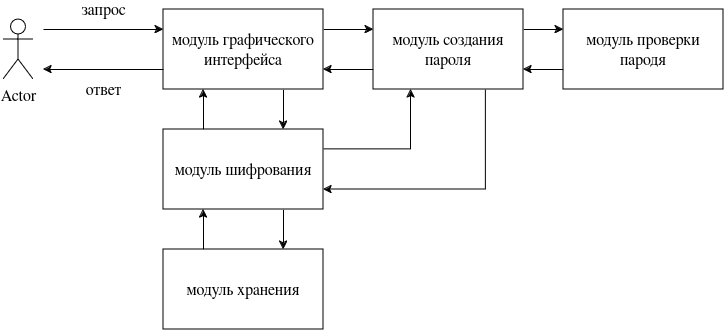
\includegraphics[width=\textwidth]{assets/shema.png}
                \caption{QR-код с ссылкой на исходный код}
            \end{figure}
        }
        

        \item {
            В приложение были загружены следующие данные:
            \begin{figure}[H]
                \centering
                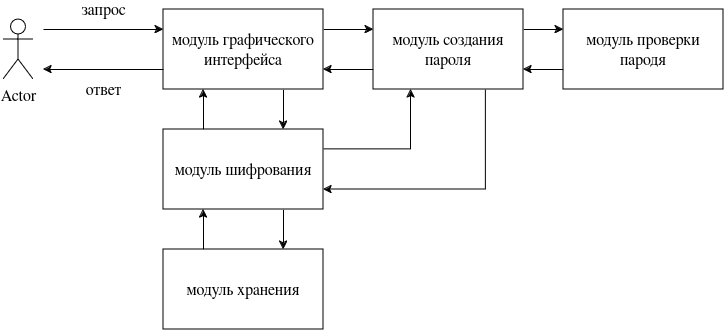
\includegraphics[width=\textwidth]{assets/shema.png}
                \caption{QR-код с ссылкой на исходный код}
            \end{figure}
        }
    \end{enumerate}

}
\newcommand{\conclusion}{
    реализовали интеллектуальную систему.
}
